\chapter{Modelado 3D Básico}

\begin{figure}[H]
	\centering
	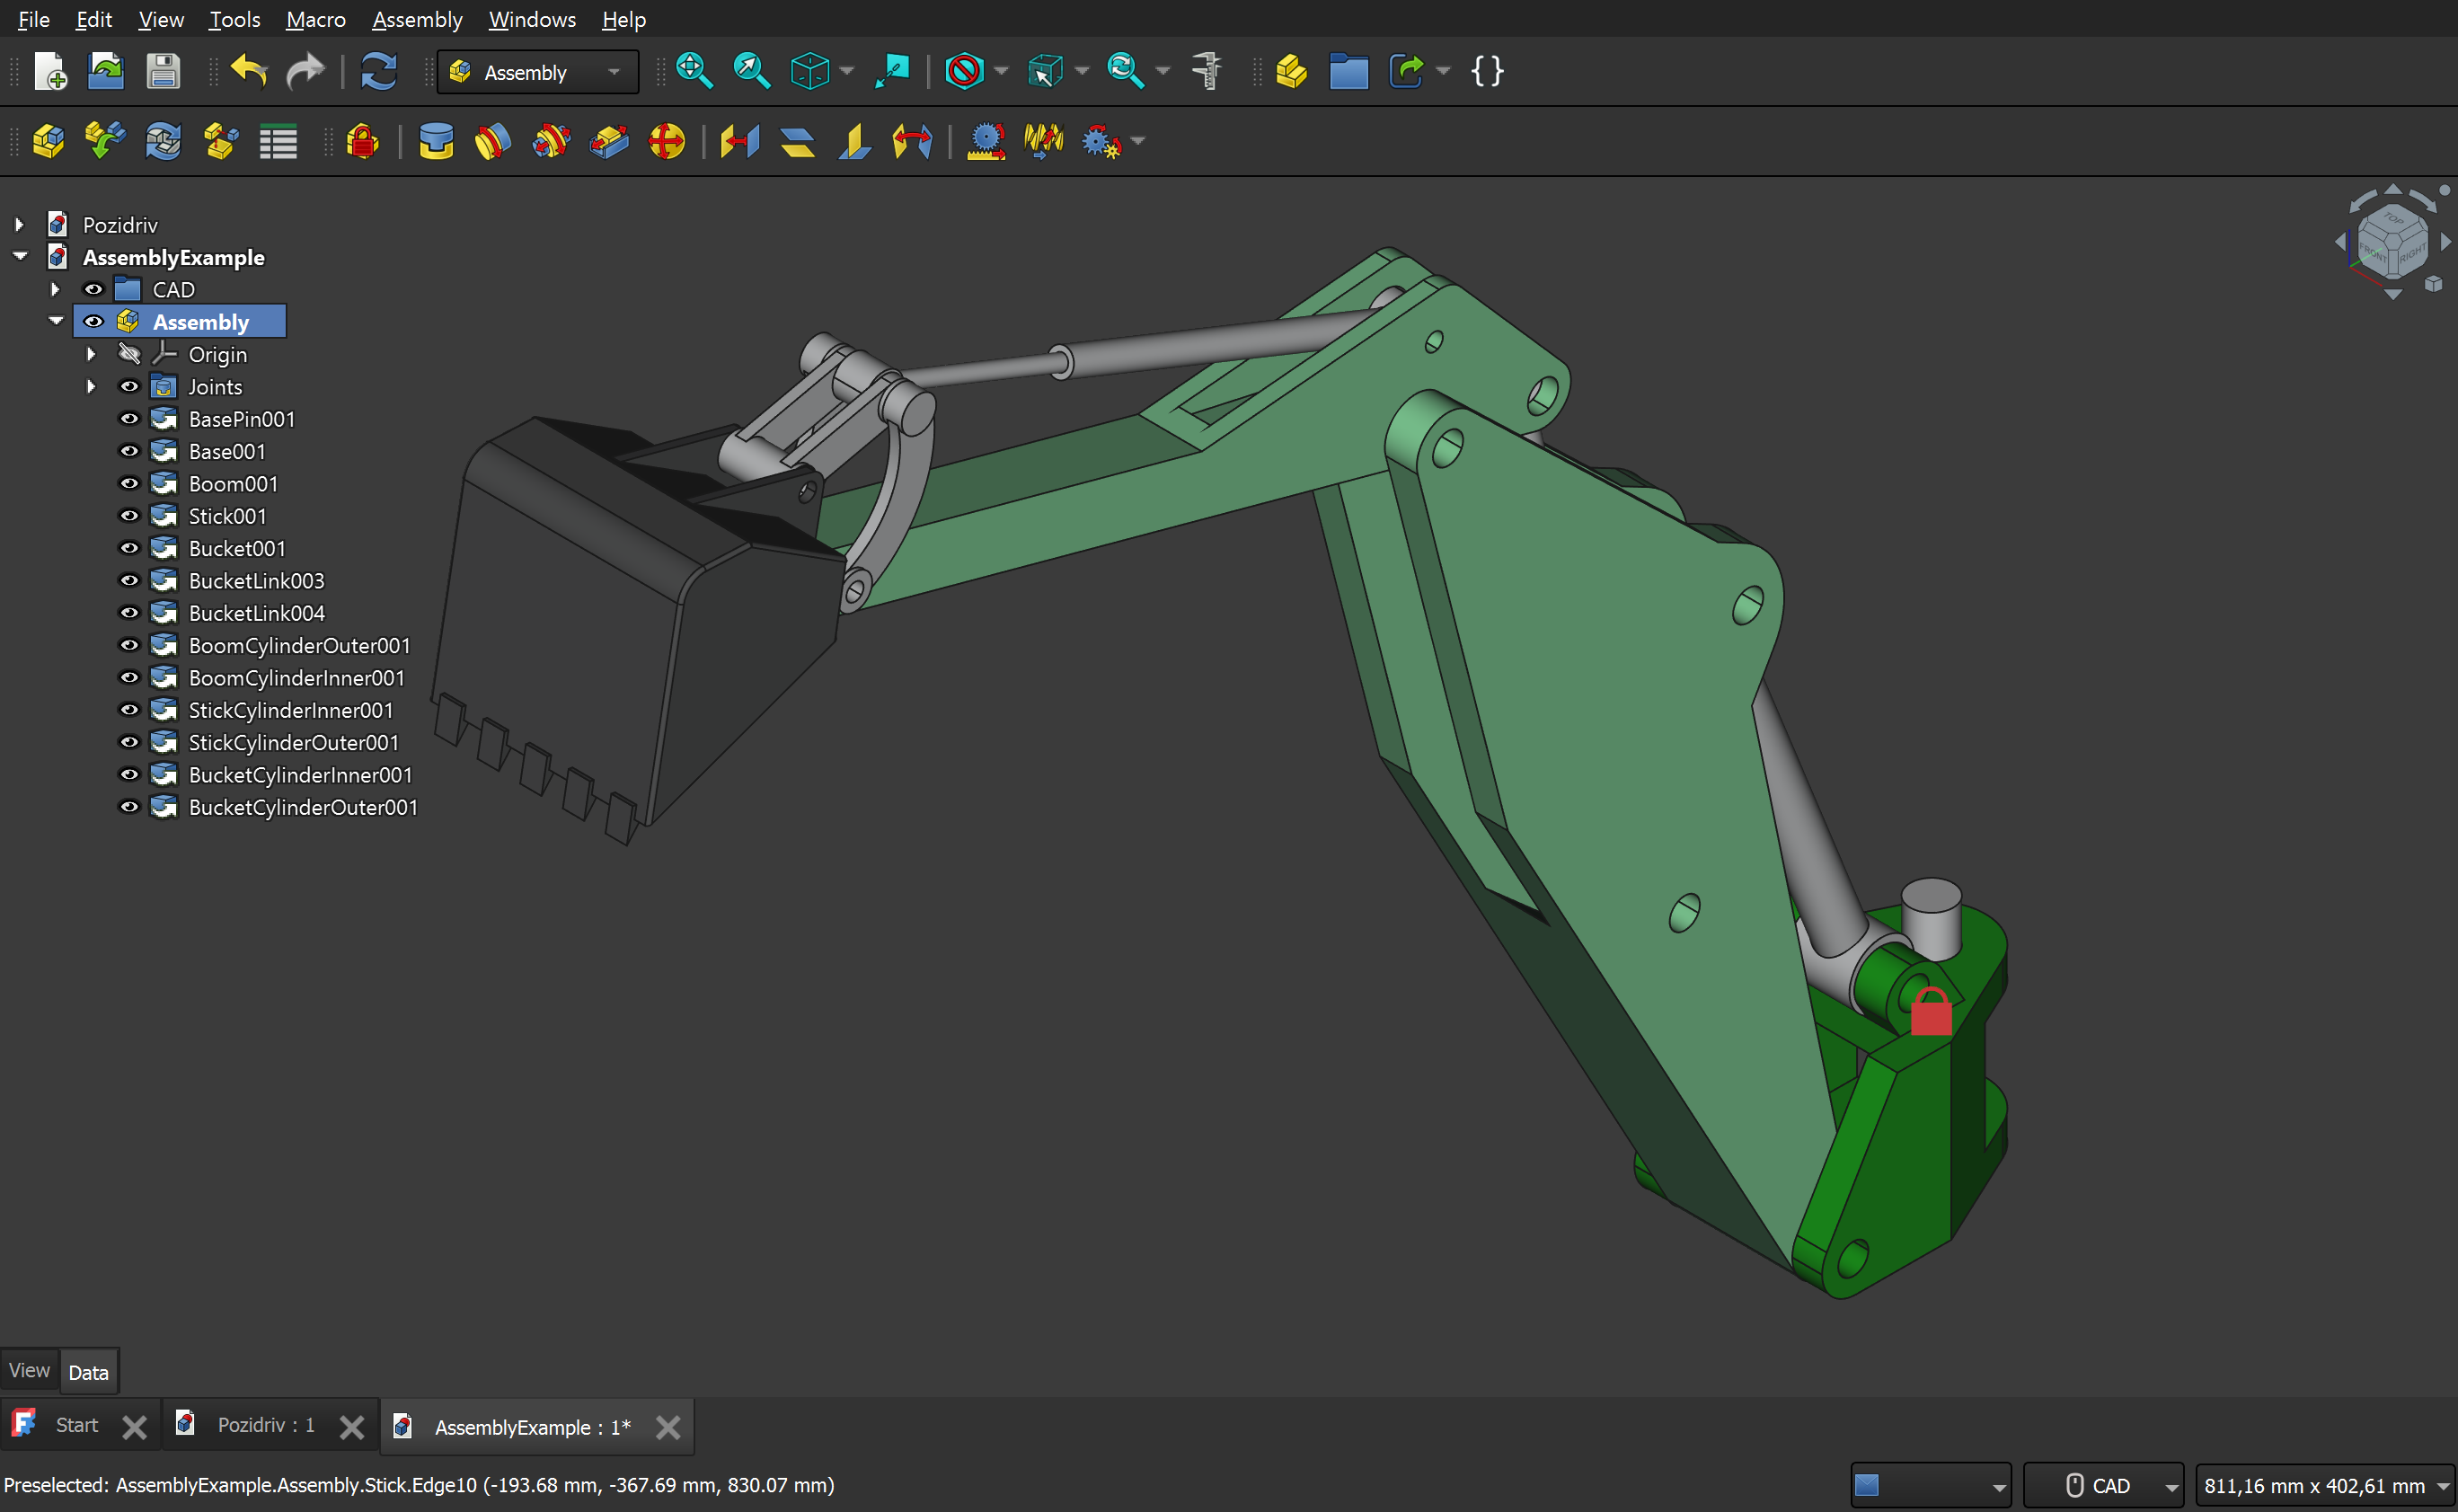
\includegraphics[width=0.8\textwidth]{img/cap4_modelado3d.png}
	\caption{Modelo 3D de ensamblaje creado en FreeCAD}
\end{figure}

Aprende los fundamentos del modelado 3D en FreeCAD.
Crea sólidos simples y entiende el concepto de
modelado paramétrico.

%% D. Búsqueda e Inserción de Activos Gráficos
%% Imagen insertada al inicio del capítulo

%% B. Actividades Teóricas
\section{Investigar y responder}
\faPencil

Investiga sobre modelado 3D en FreeCAD y responde:
\begin{enumerate}
	\item ¿Qué es el modelado sólido (solid modeling)?
	\item ¿Cuáles son las formas geométricas básicas en 3D?
	\item ¿Cómo se relacionan los bocetos 2D con los
	      sólidos 3D?
	\item ¿Qué es una operación booleana en modelado 3D?
	\item ¿Cómo se unen y separan sólidos en FreeCAD?
	\item ¿Qué significa que el modelado sea paramétrico?
	\item ¿Cómo se modifican las dimensiones después de
	      crear un sólido?
	\item ¿Qué son las características (features) en
	      FreeCAD?
\end{enumerate}

%% C. Actividades Prácticas
\section{Resolver los siguientes problemas}
\faWrench

Problemas para aplicar conocimientos:
\begin{enumerate}
	\item Crea un cubo de 50x50x50 mm usando la herramienta
	      de caja.
	\item Modela un cilindro de radio 20 mm y altura 40 mm.
	\item Crea una esfera de radio 25 mm.
	\item Modela una pieza combinando cubo y cilindro con
	      operación de unión.
	\item Crea un agujero cilíndrico en un cubo usando
	      operación de sustracción.
	\item Modela un prisma hexagonal de lado 15 mm y altura
	      30 mm.
	\item Crea una pieza con varios sólidos y guárdala como
	      archivo FreeCAD.
	\item Practica la modificación de dimensiones en un
	      modelo existente.
	\item Modela una pieza simple que simule una tuercas
	      mecánica.
	\item Exporta tu modelo a formato STEP para usar en
	      otros programas.
\end{enumerate}